\chapter{Проектирование. ПРИДУМАТЬ НАЗВАНИЕ}
\section{Настройка Node.js}
\subsection{Настройка под Linux}\label{OnLinuxInstall}
В данном разделе описывается установка Node.js на Ubuntu 11.10.
Устанавливаем сам nodejs:
\begin{lstlisting}[numbers=none, language=bash]
	$ sudo apt-get install nodejs
\end{lstlisting}
Далее устанавливаем пакетный менеджер npm (Node Package Manager):
\begin{lstlisting}[numbers=none, language=bash]
	$ sudo apt-get install npm
\end{lstlisting}
Перед установкой node-ffi должен быть установлен Python (он уже по умолчанию стоит на Ubuntu 11.10). Если требуется установка, то также используется пакетный менеджер (рекомендуемая версия Python 2.7.2).
Также должен быть установлен C/C++ компилятор, например, gcc:
\begin{lstlisting}[numbers=none, language=bash]
	$ sudo apt-get install gcc
\end{lstlisting}
После предварительных установок устанавливаем node-ffi:
\begin{lstlisting}[numbers=none, language=bash]
	$ npm install ffi
\end{lstlisting}
Если установка не прошла успешна, а все предыдущие шаги были выполнены верно, то значит в операционной система используется библиотека libffi не той версии, которая нам нужна. Такая проблема возникла в Ubuntu 11.10. При установке на Ubuntu 12.04 такой проблемы нет. Соответственно тогда удаляем старую библиотеку:
\begin{lstlisting}[numbers=none, language=bash]
	$ sudo apt-get remove libffi4
\end{lstlisting}
И устанавливаем  (libffi-dev, если libffi нет):
\begin{lstlisting}[numbers=none, language=bash]
	$ sudo apt-get install libffi
\end{lstlisting}
После этого снова повторяем установку node-ffi.
\subsection{Настройка под Windows}
Для установки Node.js достаточно скачать установщик с официального сайта программы (nodejs.org) и установить его. На данном этапе проекта подключить node-ffi в Windows не удалось. 
Далее представлены испробованные способы установки.
\paragraph{Установка, используя документацию, приложенную к библиотеке node-ffi.}
Предварительно под Windows нужно установить python 2.7.2, также Microsoft Visual Studio C++, разработчики рекомендуют последнюю версию на данный момент, а именно Visual C++ 2010 Express. Также для 64-х битных систем нужно установить Windows 7 64-bit SDK.
После установки всего в командной строке была произведена попытка установки node-ffi через npm (npm install node-ffi). На рис. ~\ref{sh_error} представлена ошибка, возращаемая при таком способе установки. 
\begin{figure}[!ht]
	\begin{center}
		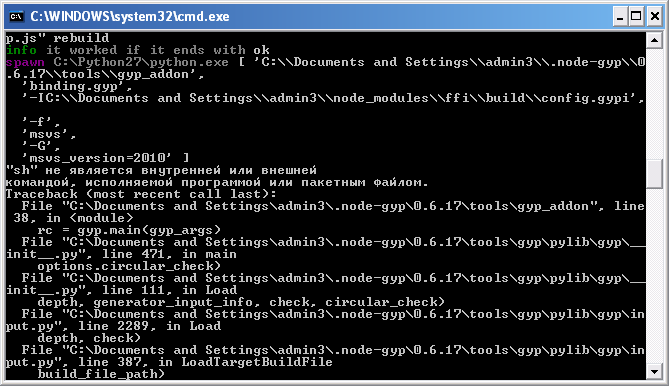
\includegraphics[width=11cm]{SH_error}
	\end{center}
	\caption{Ошибка при установке node-ffi через npm в командной строке}
	\label{sh_error}
\end{figure}
SH — Shell Script — скрипт, в котором представлены наборы команд для последовательного выполнения команд в командной строк Unix-подобных систем. Соответственно, под Windows данная команд на выполнение скрипта не будет выполняться.
\newpage

\paragraph{Установка с помощью "Установщика веб-платформы".}
Данная программа является аналогом пакетного менеджера в Unix-подобных системах. Скачать её можно на сайте: http://www.microsoft.com/web/downloads/platform.aspx (рис. ~\ref{installer_web})
\begin{figure}[!ht]
	\begin{center}
		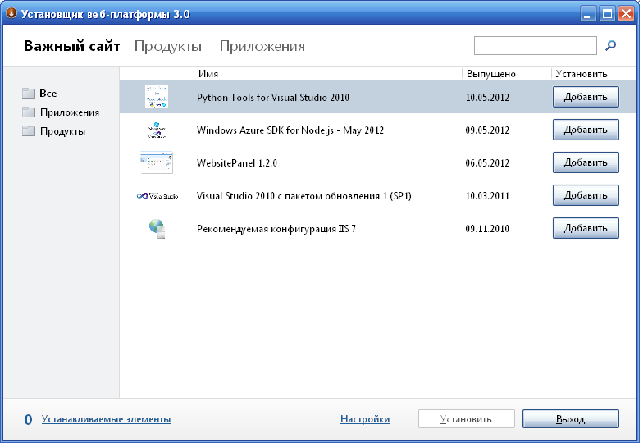
\includegraphics[width=11cm]{installer_web}
	\end{center}
	\caption{Установщик веб-платформы 3.0}
	\label{installer_web}
\end{figure}
Для установки node.js через установщик нужно установить рабочее окружение. 
Устанавливаем рекомендуемую конфигурацию IIS 7. 
Заходим в Настройки и добавляем сайт, на котором можно скачать nodejs:  http://www.helicontech.com/zoo/feed (рис. ~\ref{properties_web}).
\begin{figure}[!ht]
	\begin{center}
		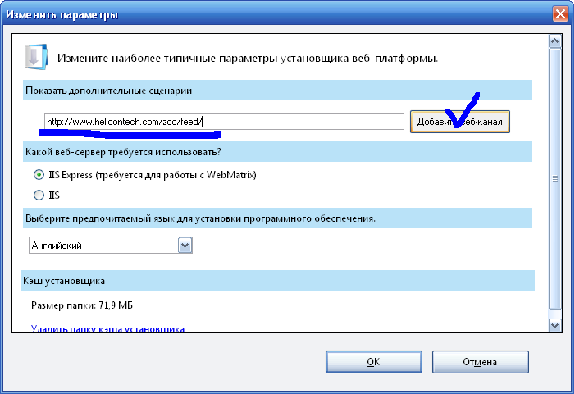
\includegraphics[width=11cm]{properties_web}
	\end{center}
	\caption{Добавление сайта, содержащего пакет установки Node.js}
	\label{properties_web}
\end{figure}
После этого на вкладке Zoo устанавливаем в разделе Packages, как показано на рис. ~\ref{package_web}.
\begin{figure}[!ht]
	\begin{center}
		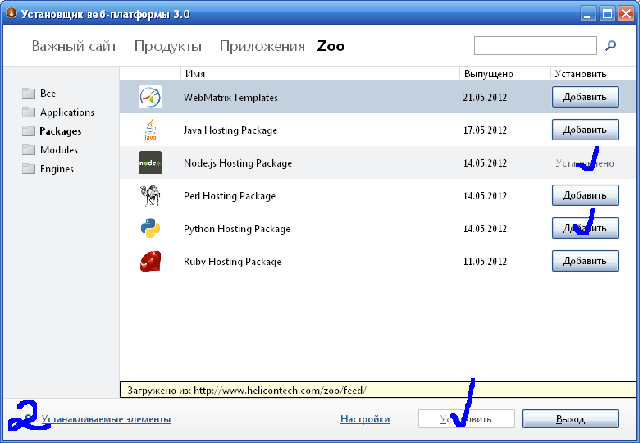
\includegraphics[width=11cm]{package_web}
	\end{center}
	\caption{Установка требуемых пакетов}
	\label{package_web}
\end{figure}
Далее устанавливаем WebMatrix Templates. На рис. ~\ref{fail_install} отображена возвращающаяся ошибка при установке.
\begin{figure}[!ht]
	\begin{center}
		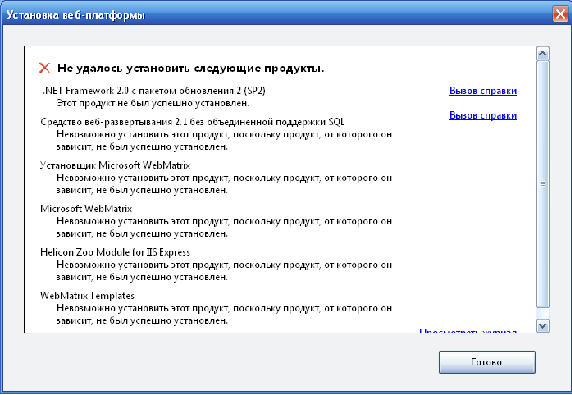
\includegraphics[width=11cm]{fail_install}
	\end{center}
	\caption{Возвращаемая ошибка}
	\label{fail_install}
\end{figure}
Никаких советов по исправлению этой проблемы найти не удалось. Установка таким способом пробовалась на Windows XP sp2 x64, sp3 x64 и x86. При удалении текущих версий .NET Framework никаких положительных изменений не происходило.  
Поэтому данный метод  также оказался неудачным.

\paragraph{Установка Node.js через Cygwin.}
Далее появилась идея избежать ошибки, выдаваемой командной строкой об sh, установкой node-ffi через Cygwin. 
Cygwin — UNIX-подобная среда и интерфейс командной строки для Microsoft Windows. Cygwin обеспечивает тесную интеграцию Windows приложений, данных и ресурсов с приложениями, данными и ресурсами UNIX-подобной среды. Из среды Cygwin можно запускать Windows приложения, также можно использовать инструменты Cygwin из Windows.

Cygwin состоит из двух частей: динамически подключаемая библиотека cygwin1.dll, которая обеспечивает совместимость API и реализует значительную часть стандарта POSIX и огромная коллекция приложений, которые обеспечивают привычную среду UNIX.

Стандарт Posix – это один из общепринятых стандартов повышения мобильности программного обеспечения (ПО).  Задача обеспечения мобильности ПО является очень важной задачей исключительной сложности. Едва ли стоит обосновывать это каким-либо более широким способом.
При установке Cygwin в каталог собирается Linux-подобный корневой каталог, представленный на рис. ~\ref{cygwin_catalogue}.
\begin{figure}[!ht]
	\begin{center}
		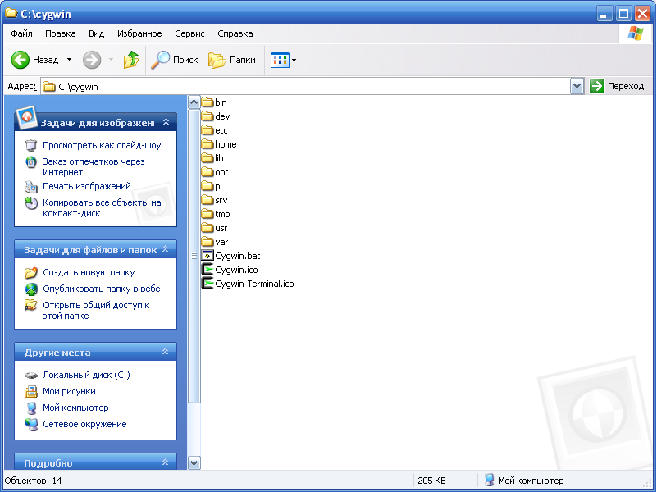
\includegraphics[width=11cm]{cygwin_catalogue}
	\end{center}
	\caption{Корневая папка Cygwin}
	\label{cygwin_catalogue}
\end{figure}

	При запуске Cygwin-Terminal открывается Terminal как в Linux, соответственно, если в его окружение установить всё, что надо (смотри пункт ~\ref{OnLinuxInstall}), то должен установиться node-ffi. Но возникла проблема с тем, что установка libffi тянет за собой, грубо говоря, весь Linux. Очень много времени было потрачено на попытки установки node-ffi через Cygwin, но результат не был достигнут.
\paragraph{Подведение итогов.} На данный момент решение данной проблемы придумано не было. Создателем платформы был отправлен запрос на помощь в установке node-ffi с подробным описанием проблем в установке.\\
Буквально на днях был получен ответ, в котором было сказано попробовать установить всё через Mozilla-Build, при этом скомпилировав в ней libffi. В условиях сдачи диплома на данный момент времени попробовать такой вариант нет. Работа над установкой node-ffi под Windows будет продолжена позднее.  Вообще говоря, большое количество программистов, использующих node.js сетуют на Node Package Manager, потому что он требует серьёзных предустановок и даже при этом не работает стабильно. \\
Существует предложение создать уже скомпилированные файлы для установки под каждую версию операционных систем, для того, чтобы не нужно было устанавливать такое большой объем программ. Кстати, в рамках нашего проекта, это может послужить большой проблемой, размещая сервер локально на каждом компьютере, будет необходимо установить большой объём информации. С одной стороны технология использования Node.js пока что не оправдала себя полностью , но ещё есть более полугода, возможно, разработчики исправят эту проблему, либо придётся компилировать всё своими руками. С другой стороны размещение сервера удалённо решит эту проблему  и тут node.js, как уже было описано, подходит как нельзя кстати.\\
Нет волнений, что текущая идея может быть невыполнима, используя выбранные технологии.
